\section{系统实现}\label{implement}
本文使用Python与C++实现该算法。八叉树相关实现,如分配,索引,求交运算,采样等使用C++完成, Python中主要实现了IncrementalMapping与GlobalMapping两个类。为实现两个线程共享数据,本文使用Python多线程管理工具multiprocessing.managers进行通讯,将地图体素,地图特征,关键帧集合与解码器及其参数共享,使得两个线程能够对上述数据进行同步更新。两个主要线程算法的伪代码如算法\ref{incrementalmapping}和算法\ref{globalmapping}所示。
\begin{algorithm}
    \caption{增量建图}\label{incrementalmapping}
    \begin{algorithmic}[1]
      \Require
        包含位姿和语义信息的点云帧集合$S_{frame}$
      \Ensure
        体素集合$S_{voxel}$;
        地图特征集合$S_{feature}$;
        解码器网络参数$\theta, \phi$;
        关键帧集合$S_{keyframe}$
      \Function{IncrementalMapping}{$S_{frame}$}
      \For{each $frame\in S_{frame}$}
      \State $S_{voxel}\gets S_{voxel}+$ \Call{CreateVoxel}{$frame$}
      \State $S'_{feature}, \theta', \phi'\gets$\Call{Mapping}{$frame$}
      \State $S_{feature},\theta,\phi\gets$\Call{UpdateSharedData}{$S'_{feature}, \theta', \phi'$}
      \If{\Call{IsKeyFrame}{$frame$}}
      \State $S_{keyframe}\gets S_{keyframe}+frame$
      \EndIf
      \EndFor
      \State \Return{$S_{voxel},S_{feature},\theta,\phi,S_{keyframe}$}
      \EndFunction

      \Function{Mapping}{$frame$}
      \State $rays \gets$\Call{SampleRays}{$frame$}
      \For{each $ray\in rays$}
      \If{\Call{IsIntersect}{$ray,S_{voxel}$}}
      \State $points\gets$\Call{SamplePoints}{$ray$}
      \State \Call{Render}{$points,S_{feature},\theta,\phi$}
      \State $S'_{feature}, \theta', \phi'\gets$\Call{Optimize}{$S_{feature}, \theta, \phi$}
      \EndIf
      \EndFor
      \State \Return{$S'_{feature}, \theta', \phi'$}
      \EndFunction
    \end{algorithmic}
\end{algorithm}
\begin{algorithm}
    \caption{全局建图}\label{globalmapping}
    \begin{algorithmic}[1]
      \Require
        关键帧集合$S_{keyframe}$
      \Ensure
        体素集合$S_{voxel}$;
        地图特征集合$S_{feature}$;
        解码器网络参数$\theta, \phi$;
        
      \Function{GlobalMapping}{$S_{keyframe}$}
      \State$optimizeTargets\gets$\Call{RandomSelectFrames}{$S_{keyframe}$}
      \State $S'_{feature}, \theta', \phi'\gets$\Call{Mapping}{$optimizeTargets$}
      \State $S_{feature},\theta,\phi\gets$\Call{UpdateSharedData}{$S'_{feature}, \theta', \phi'$}
      \State \Return{$S_{voxel},S_{feature},\theta,\phi,S_{keyframe}$}
      \EndFunction
    \end{algorithmic}
\end{algorithm}
\clearpage
\section{实验}\label{numerical experiments}
\subsection{地图提取}
本文使用训练完毕的地图特征与解码器进行推理并导出地图的顶点与面元数据,以网格格式对结果进行评估。对于网格中每一个被分配的体素,本文将其再次细分为$N \times N \times N$个部分,直接推理出其内部$N^3$个点的SDF值和语义信息。如图\ref{marching}所示最终使用marching cubes\cite{marchingcubes}等值面提取算法提取出地图的所有顶点与表面,并将语义信息映射为顶点颜色。
\begin{figure}[htbp]
    \centering
    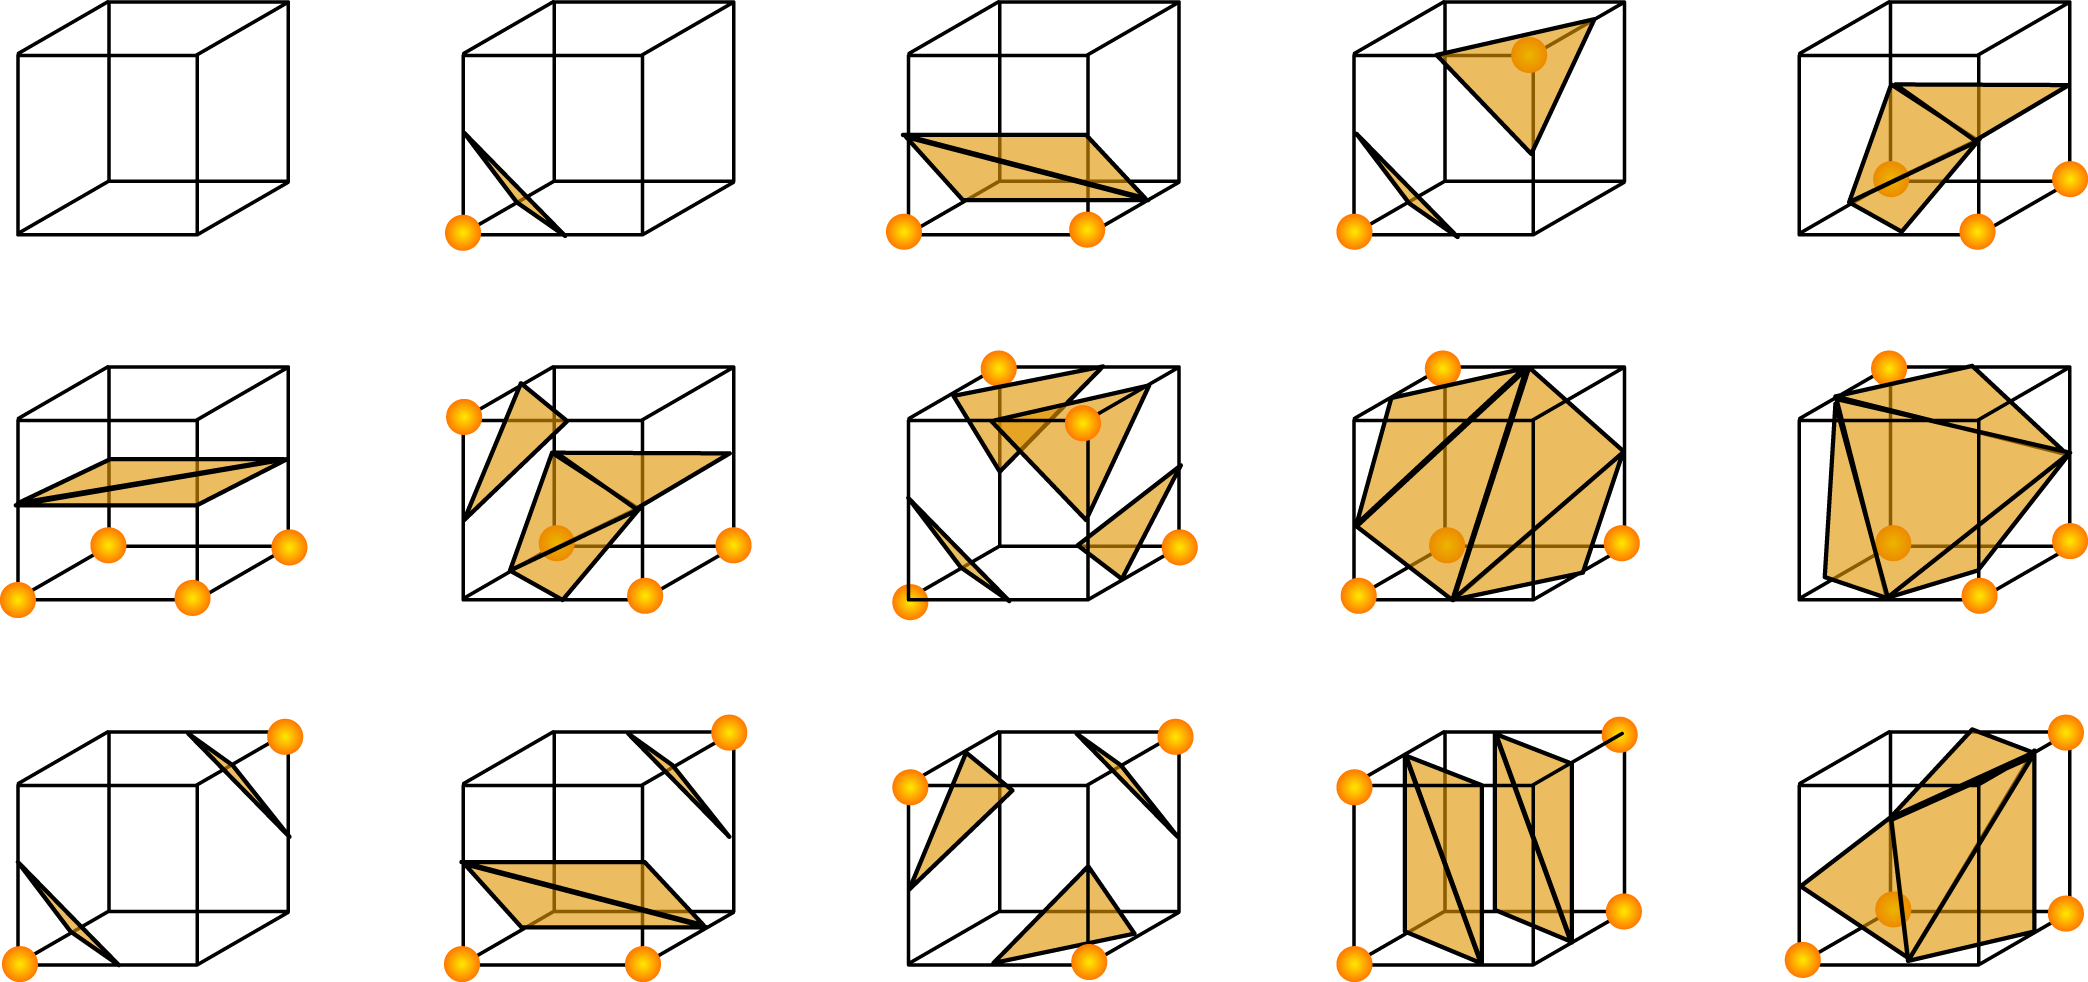
\includegraphics[scale=0.7]{figures/MarchingCubes.png}
    \caption{marching cube算法,图源维基百科\cite{marchingpicture}。首先将空间划分为立方体网格,根据顶点处数值与等值面的关系将立方体分为14种状态。最后根据等值面穿过边的状态生成相应的三角片元。}\label{marching}
\end{figure}
\subsection{评价指标}
为评价重建地图的几何精度,本文使用KD树\cite{kd}(K-Dimension Tree)和KNN(K-Nearest Neighbors)\cite{knn}算法分别从两组顶点数据中计算最邻近点的距离,并使用以下5个指标对重建结果进行评价:距离误差,准确率,召回率,L1倒角距离(Chamfer-L1)和F1-score。进一步,我们将距离误差称为完成度(Completeness),将召回率称为完成率(Completeness Ratio)。

完成度指的是Ground Truth中每个点与其预测结果中的对应点的平均距离。Chamfer-L1距离,也称为曼哈顿倒角距离或L1倒角距离,用于衡量两个集合之间的最短距离。其计算方式是取目标形状的每个边缘点或曲线上的点与参考形状的边缘点或曲线上的点曼哈顿距离后计算平均值或求和。本文设置了一个阈值$threshold$以表示两个点是否重合,若两点距离$d<threshold$,则表示两者重合,即重建成功。使用该方法得出重建结果的准确率与召回率。

具体地说,对于Ground Truth顶点集合与由本文方法重建出的顶点,我们分别对其进行下采样得到顶点集合$V_{gt}$和$V_{pred}$。我们对$V_{gt}$中的每一个顶点执行KNN算法,找到其到$V_{pred}$中最近点的距离,得到一个距离集合$D_{r}$。同样的,我们对$V_{pred}$中的每一个点找到其在$V_{gt}$中距离最近的点,将其距离记录为$D_{p}$。上述各项指标的计算公式如下所示:
\begin{equation*}
\begin{alignedat}{2}
D'_{p} &= \{d \in D_{p} \mid d < threshold\}\;,\\
D'_{r} &= \{d \in D_r\mid d<threshold\}\;,\\
Completeness &= \frac{1}{|D_{r}|}\sum_{i=0}^{|D_{r}|}D_{r}[i]\;\\
Accuracy&= \frac{1}{|D'_{p}|}\sum_{i=0}^{|D'_{p}|}D'_{p}[i]\;,\\
Recall &=\frac{1}{|D'_{r}|}\sum_{i=0}^{|D'_{r}|}D'_{r}[i]\;,\\
Chamfer\_L1 &= \frac{1}{2}\left(Completeness + \frac{1}{|D_{p}|}\sum_{i=0}^{|D_{p}|}D_{p}[i]\right)\;,\\
F1\_score &= \frac{2\times Accuracy\times Recall}{Accuracy + Recall}
\end{alignedat}
\end{equation*}
\subsection{实验准备}
\subsubsection{数据集}
本文的方法在3个公开的户外激光雷达数据集上进行了定性和定量的测试:(1)人工合成的MaiCity数据集\cite{maicity},模拟使用64线无噪声激光雷达对城市场景扫描序列组成。(2)真实世界的Newer College数据集\cite{ncd},该数据集在牛津大学内使用手持激光雷达记录,具有厘米级测量噪声和大量运动失真。其地面数据使用地面扫描仪获得。两者均带有地面附近的Ground Truth网格数据用作评估。(3) KITTI\cite{KITTI}是目前最大的自动驾驶场景下的计算机视觉算法评测数据集,SemanticKITTI\cite{SemanticKITTI}为其点云数据标注了语义信息。其数据包括激光雷达与RGB-D数据流等,每一帧中出现多个车辆或行人,包含超过20种语义标签类型。
\subsubsection{实验配置}
本文中的两个解码器均为两层全连接层,其中SDF解码器每层有128个节点,语义解码器有256个节点。对于每一帧数据采样1024个点进行训练,设定关键帧窗口大小为5。对于不同的数据集,本文使用表\ref{parameters}中设定的超参数进行训练:
\begin{table}[htbp]
    \centering
    \caption{}\label{parameters}
    \begin{tabular}[htbp]{llcccc}
        \toprule
        \multicolumn{2}{l}{数据集} & 体素大小(m) & 采样间距(m) & 截断距离(m) &最大碰撞体素数 \\
        \midrule
        \multicolumn{2}{l}{KITTI} & 0.4 & 0.2 &0.3 &10\\
        \multicolumn{2}{l}{Mai City} & 0.2 \\
        \multicolumn{2}{l}{New College} & 0.2 \\
        \bottomrule
    \end{tabular}
\end{table}
\subsection{实验结果}
sdfloss+depthloss 和只有bceloss的对比
有无replay机制的对比
\subsubsection{合成场景}
\subsubsection{真实场景}
\subsection{算法时间与内存占用}
% 本节分别使用鲲鲲内卷法,中中内卷法,伟伟内卷法进行时间比较。在3天内,让实验组和对照组分别在3天内写论文。鲲鲲卷卷法3天写出了一篇CVPR,中中卷卷法3天写出了一篇AAAI,对照组三天写出了一份10页报告,而伟伟卷卷法3天从黄铜上分到了白银。

% \begin{figure}[hb!]
%     \centering
%     \subfigure[目标检测]{
%     \begin{minipage}[t]{0.22\linewidth}
%     \centering
%     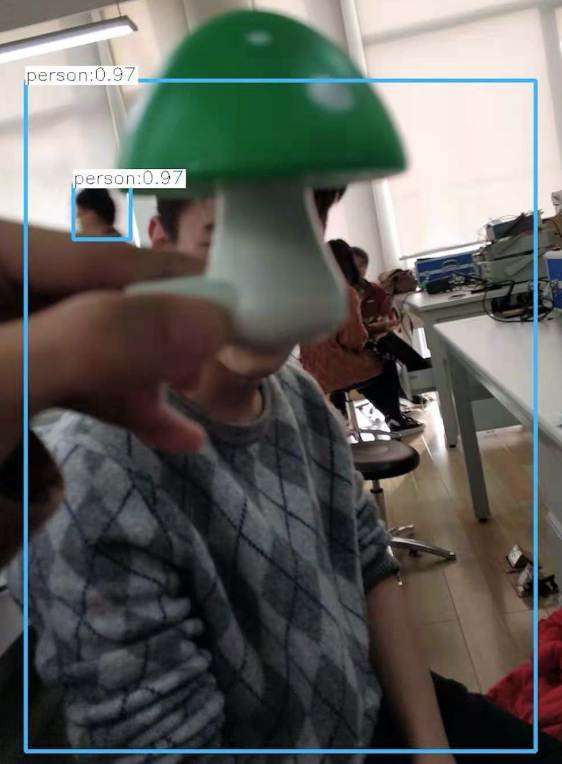
\includegraphics[width=\linewidth]{figures/det.png}
%     \end{minipage}\label{fig:det}
%     }
%     %
%     \centering
%     \subfigure[语义分割]{
%     \begin{minipage}[t]{0.28\linewidth}
%     \centering
%     
\includegraphics[width=\linewidth]{figures/seg.png}
%     \end{minipage}\label{fig:seg}
%     }
%     %
%     \centering
%     \subfigure[姿态识别]{
%     \begin{minipage}[t]{0.4\linewidth}
%     \centering
%     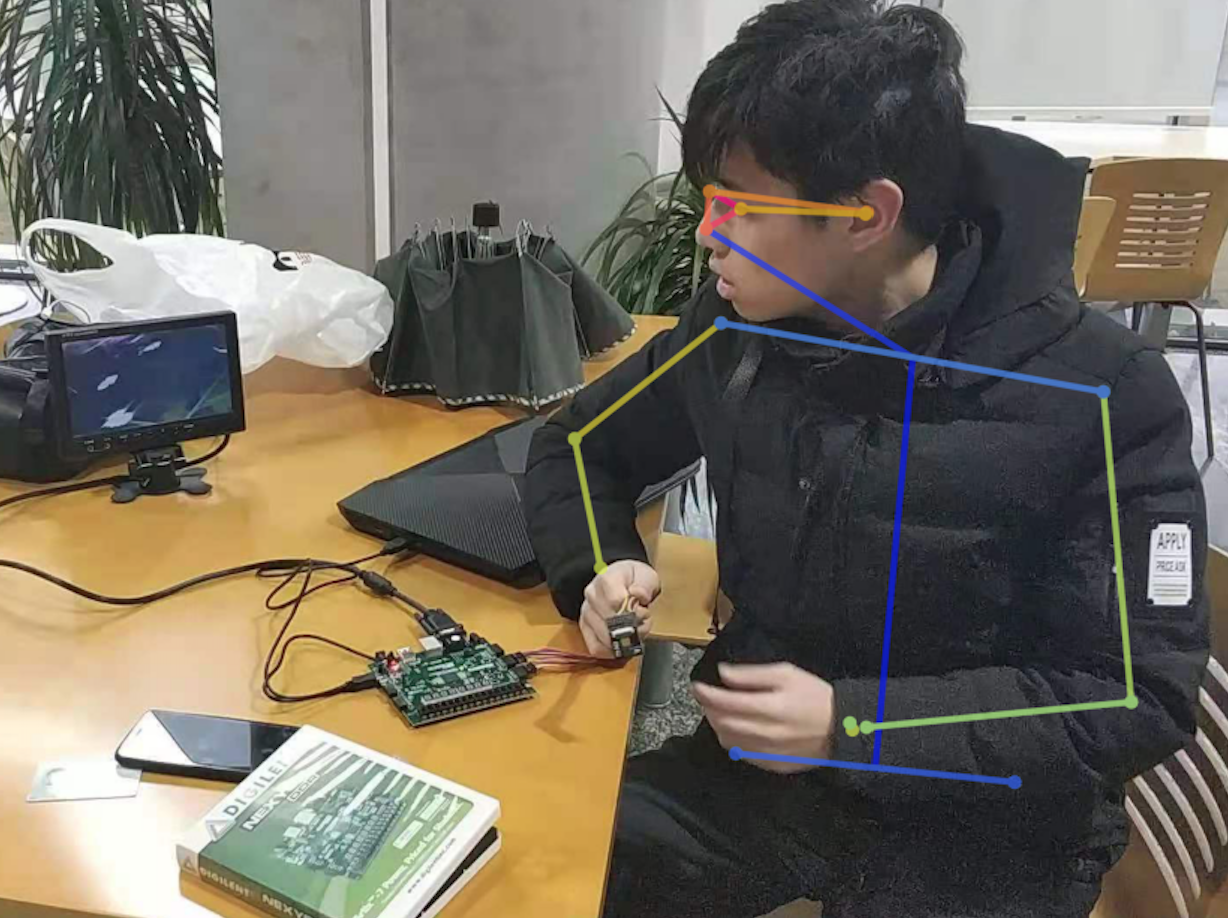
\includegraphics[width=\linewidth]{figures/pose.png}
%     \end{minipage}\label{fig:pose}
%     }
%     %
%     \caption{常见视频分析应用图解(图片提供者为中中同学)}\label{fig:cvexample}
%     \centering
% \end{figure}